\subsection{The Packfile}
This chapter explains in detail, down to the bits, how the packfile and pack
index files are formatted.

\subsubsection{The Packfile Index}
First off, we have the packfile index, which is basically just a series of
bookmarks into a packfile.

There are two versions of the packfile index - version one, which is the
default in versions of Git earlier than 1.6, and version two, which is the
default from 1.6 forward, but which can be read by Git versions going back to
1.5.2, and has been further backported to 1.4.4.5 if you are still on the 1.4
series.

Version 2 also includes a CRC checksum of each object so compressed data can be
copied directly from pack to pack during repacking without undetected data
corruption. Version 2 indexes can also handle packfiles larger than 4 Gb. See
figure \ref{fig:packfileindex} on page \pageref{fig:packfileindex}
\begin{figure*}[tbp]
\centering
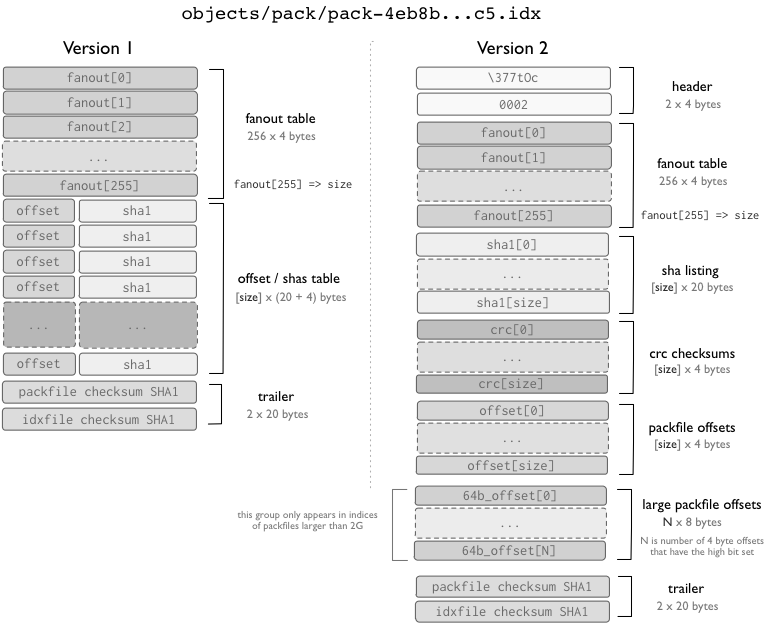
\includegraphics[width=0.80\textwidth]{content/git/packfile-index.png}
\label{fig:packfileindex}
\caption{Packfile Intex}
\end{figure*}

In both formats, the fanout table is simply a way to find the offset of a
particular sha faster within the index file. The offset/sha1 tables are sorted
by sha1 values (this is to allow binary search of this table), and fanout table
points at the offset/sha1 table in a specific way (so that part of the latter
table that covers all hashes that start with a given byte can be found to avoid
8 iterations of the binary search).

In version 1, the offsets and shas are in the same space, where in version two,
there are seperate tables for the shas, crc checksums and offsets. At the end
of both files are checksum shas for both the index file and the packfile it
references.

Importantly, packfile indexes are not neccesary to extract objects from a
packfile, they are simply used to quickly retrieve individual objects from a
pack. The packfile format is used in upload-pack and receieve-pack programs
(push and fetch protocols) to transfer objects and there is no index used then
- it can be built after the fact by scanning the packfile.

\subsubsection{The Packfile Format}
The packfile itself is a very simple format. There is a header, a series of
packed objects (each with it's own header and body) and then a checksum
trailer. The first four bytes is the string 'PACK', which is sort of used to
make sure you're getting the start of the packfile correctly. This is followed
by a 4-byte packfile version number and then a 4-byte number of entries in that
file. In Ruby, you might read the header data like this:
\lstset{basicstyle=\scriptsize, numbers=none, captionpos=b, tabsize=4}
\begin{lstlisting}[caption=,language={ruby},
breaklines=true,label=lst:]
def read_pack_header
  sig = @session.recv(4)
  ver = @session.recv(4).unpack("N")[0]
  entries = @session.recv(4).unpack("N")[0]
  [sig, ver, entries]
end
\end{lstlisting}

After that, you get a series of packed objects, in order of their SHAs which
each consist of an object header and object contents. At the end of the
packfile is a 20-byte SHA1 sum of all the shas (in sorted order) in that
packfile. See figure \ref{fig:packfileformat} on page \pageref{fig:packfileformat}

\begin{figure*}[tbp]
\centering
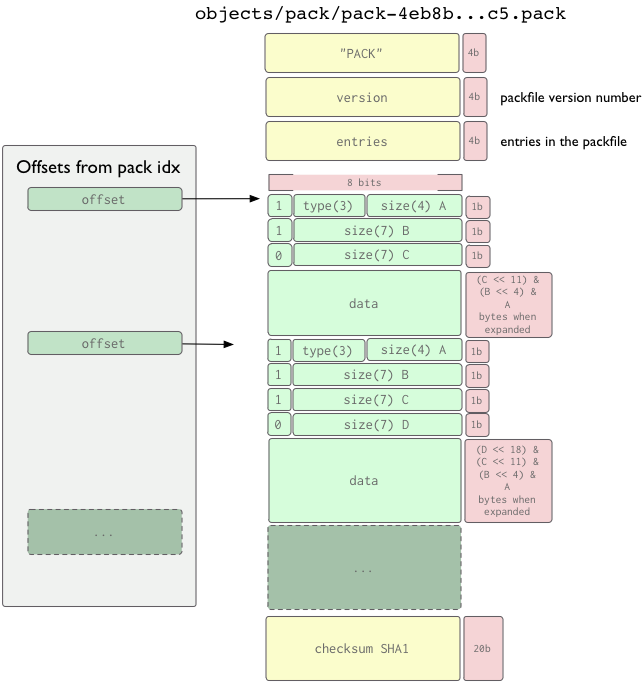
\includegraphics[width=0.80\textwidth]{content/git/packfile-format.png}
\label{fig:packfileformat}
\caption{Packfile format}
\end{figure*}

The object header is a series of one or more 1 byte (8 bit) hunks that specify
the type of object the following data is, and the size of the data when
expanded. Each byte is really 7 bits of data, with the first bit being used to
say if that hunk is the last one or not before the data starts. If the first
bit is a 1, you will read another byte, otherwise the data starts next. The
first 3 bits in the first byte specifies the type of data, according to the
table below.

(Currently, of the 8 values that can be expressed with 3 bits (0-7), 0 (000) is
'undefined' and 5 (101) is not yet used.)

Here, we can see an example of a header of two bytes, where the first specifies
that the following data is a commit, and the remainder of the first and the
last 7 bits of the second specifies that the data will be 144 bytes when
expanded. See figure \ref{fig:packfilelogic} on page \pageref{fig:packfilelogic}

\begin{figure*}[tbp]
\centering
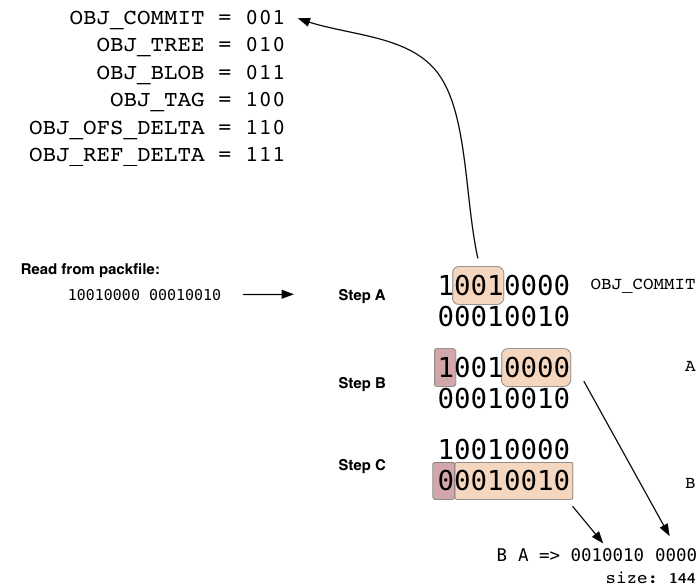
\includegraphics[width=0.80\textwidth]{content/git/packfile-logic.png}
\label{fig:packfilelogic}
\caption{Packfile logic}
\end{figure*}

It is important to note that the size specified in the header data is not the
size of the data that actually follows, but the size of that data when
expanded. This is why the offsets in the packfile index are so useful,
otherwise you have to expand every object just to tell when the next header
starts.

The data part is just zlib stream for non-delta object types; for the two delta
object representations, the data portion contains something that identifies
which base object this delta representation depends on, and the delta to apply
on the base object to resurrect this object.  ref-delta uses 20-byte hash of
the base object at the beginning of data, while ofs-delta stores an offset
within the same packfile to identify the base object. In either case, two
important constraints a reimplementor must adhere to are:

delta representation must be based on some other object within the same
packfile;

the base object must be of the same underlying type (blob, tree, commit or
tag);
